\fancyhf{}
\fancyfoot[CO, CE]{ \thepage}

\chapter{Implementation}
\label{chapter3}

\section{Design Space Exploration}

Design Space Exploration (DSE) is essential for SODA framework because it allows developers to efficiently navigate the vast array of implementation for a given application. MLIR provides a flexible infrastructure that supports multiple level of abstraction, enabling transformation and optimization of code across various stages of compilation. Furthermore, it is of great importance to identify the most efficient hardware design by evaluating different configurations of MLIR optimizations and trade-offs such as ASIC's power, performance, and area. Additionally, the diverse sizes of Convolutional Neural Networks (CNN) and Fully Connected (FC) layers have different characteristics and requires dedicated configurations for optimized hardware design. By systematically, analyzing all the possibilities, DSE helps in automating exploration of huge search space and optimizing design space. This results in reducing development time and improvement in quality of the final hardware.

\subsection{DSE Tool Flow}

\begin{figure}
    \centering
    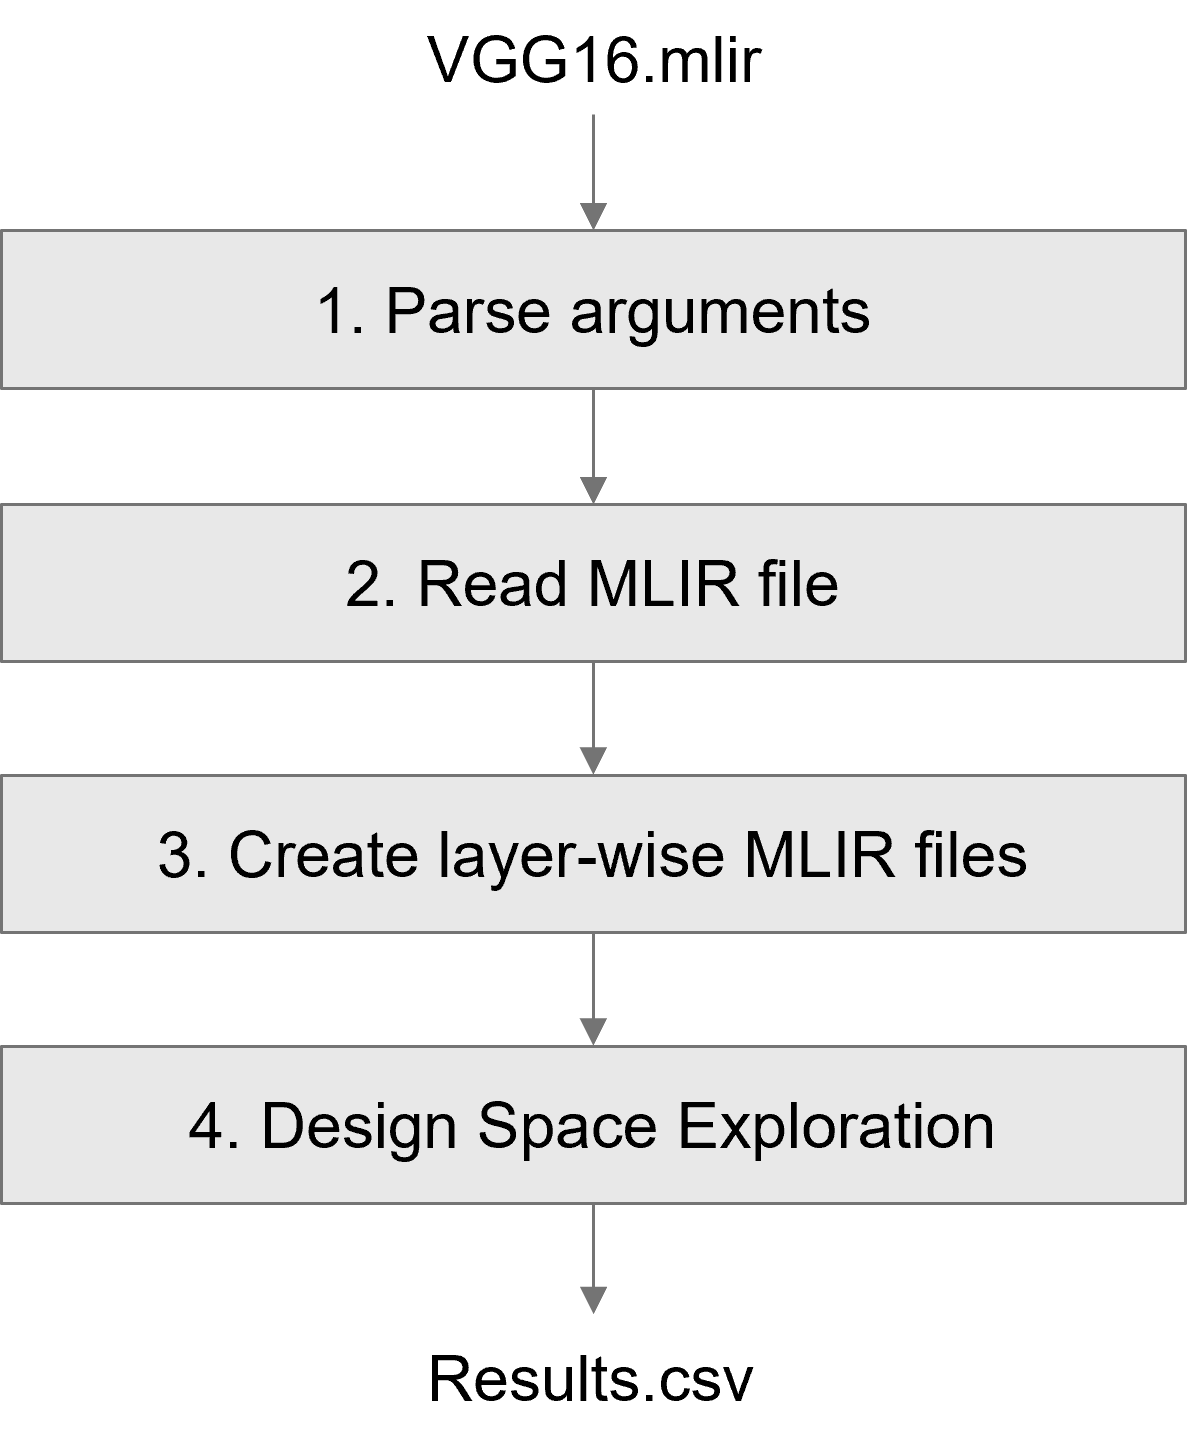
\includegraphics[width=0.4\linewidth]{figure//chapter3_implementation/Figure 1 - DSE tool flow.png}
    \caption{DSE tool flow}
    \label{fig:3.1}
\end{figure}

The Design Space Exploration (DSE) flow involves several steps to explore neural network layers:

\begin{enumerate}
    
    \item Input file: The process begins with an MLIR file, that contains all the layers of a neural network architecture at Linalg level dialect. The file serves as the input file to explore.
    
    \item Argument parsing: In this step, the type of layer (Conv2D, Depth-wise Conv2D and FC layers) and the type of loop optimization (permutation, tiling, unrolling) to explore is picked. Additionally, the layers to start or end exploration can be selected, although this is optional. The options are show in Table \ref{dseCommands}.
    
    \item Read MLIR file: At this stage, the tool reads all the layers and stores important information of all the layers. It also performs modifications to layers (discussed in subsequent sections).
    
    \item Create Temporary MLIR files: Temporary MLIR files are created for each layer with (clipped) dimensions. These layers are inserted between SODA syntax to mark the layer as an accelerated part of the code. So that SODA framework generates ASIC for the given layer.
    
    \item Design Space Exploration (DSE): This is the step that involves generating appropriate loop optimization combinations based on the characteristics of the layer. SODA, Bambu (HLS), OpenRoad (Synthesis, and Placement and routing). are executed in order to generate ASIC for a given optimization configuration of a layer. Results such as power, performance, area along with efficiency and energy are recorded.
    
    \item Output file: Finally, the results of the exploration are stored in a CSV file for further analysis and decision-making.

\end{enumerate}


\begin{table}[ht]
\caption{Table for DSE tool command-line arguments}
\centering
\resizebox{\textwidth}{!}{%
\begin{tabular}{|l|l|l|}
\hline
\textbf{Type}       & \textbf{Parameters}         & \textbf{Remarks}                  \\ \hline
\textbf{MLIR} & \texttt{--read\_mlir} & Read Neural Network MLIR file. \\ \hline
\textbf{Loop optimization} & \texttt{--permute} & Performs loop permutation. \\ \cline{2-3} 
                           & \texttt{--tile}    & Performs loop tiling. \\ \cline{2-3} 
                           & \texttt{--unroll}  & Performs loop unrolling. \\ \hline
\textbf{Type of NN layer}  & \texttt{--conv2d}  & Explores 2D Convolution layers. \\ \cline{2-3} 
                           & \texttt{--depthwise\_conv2d} & Explores 2D Depth-wise Convolution layers. \\ \cline{2-3} 
                           & \texttt{--matmul}  & Explores Fully Connected layers. \\ \hline
\textbf{Layer options (optional)} & \texttt{--start\_layer} & Select layer number to start exploring from. \\ \cline{2-3} 
                           & \texttt{--end\_layer} & Select layer number to end exploring at. \\ \cline{2-3} 
                           & \texttt{--select\_layer} & Select a particular layer to explore. \\ \hline
\end{tabular}
}
\label{dseCommands}
\end{table}

\subsection{Optimizations}
\subsubsection{Loop Optimizations:}
Loop optimizations are performed by altering the structure of the loop. Key methods are:
\begin{enumerate}
    \item Loop permutation: It is the process of swapping the order of nested loops. In matrix multiplication, permuting the loops can enhance data locality, making memory access more efficient. 
    \item Loop tiling: It is a technique that breaks down a large loop into smaller blocks or tiles. The goal is to fit these smaller blocks into memory, thereby improving memory usage and reducing memory access times.
    \item Loop unrolling: It involves expanding the loop body by replicating the operations for multiple iterations and reducing the number of iterations. This reduces the overhead associated with loop control and enables better instruction-level parallelism.
\end{enumerate}

\subsubsection{Memory Optimizations:}
Memory optimizations focus on improving data handling and access speeds. Key methods are: 
\begin{enumerate}  
    \item Affine data copy generate: It involves creating copies of specific data chunks into local memory buffers, usually to optimize for locality. By doing this, the data is brought closer to the computation, improving performance.
    \item Promote buffers to stack: It is an optimization that moves heap-allocated memory (or buffers that are globally or dynamically allocated) into stack-allocated memory. Stack allocations are typically faster as stack allocations are often in contiguous memory regions.
    \item Affine scalar replacement: It helps in reducing memory traffic by promoting scalar values, stored in memory, into registers. This is particularly beneficial when the same scalar value is used multiple times in a loop, thus improving performance by lowering the number of memory accesses.

\end{enumerate}

All the memory optimizations may not be used for every loop optimization. This is discussed in further sections.

\clearpage
\subsection{Types of Neural Network Layers}

As part of this exploration, 3 different types of neural network layers are examined.
They are 2D Convolution, 2D Depth-wise convolution, and Fully Connected layers.

\subsubsection{2D Convolution (CNN) Layer:}

2D CNN layer in MLIR is represented by \textit{'linalg.conv\_2d\_nhwc\_hwcf'} as shown in Listing \ref{lst:conv2dLinalg}. The Linalg layer has details such as dilations, strides, input feature map size, kernel size, and output feature map size. Features of the layer are shown in Fig. \ref{fig:cnnFeatures}.

The Listing \ref{lst:conv2dAffine} shows 7 nested for loops are required for CNN layer. The first loop is for batch number. Loop 2 \& 3 are output height and width respectively.  Loop 4 represents number of output channels. Loop 5 \& 6 represents kernel height \& width respectively. Loop 7 is for number of input channels.

\begin{lstlisting}[caption={Example conv2d at Linalg dialect}, label={lst:conv2dLinalg}]
linalg.conv_2d_nhwc_hwcf 
{dilations = dense<1>: tensor<2xi64>, strides = dense<4>: tensor<2xi64>}
ins(%arg0, %arg1 : memref<1x227x227x3xf32>, memref<11x11x3x96xf32>)
outs(%arg2 : memref<1x55x55x96xf32>)
}
\end{lstlisting}

\begin{lstlisting}[caption={Example conv2d at Affine dialect}, label={lst:conv2dAffine}]
affine.for %arg3 = 0 to 1 { // Loop 1
  affine.for %arg4 = 0 to 55 { // Loop 2
    affine.for %arg5 = 0 to 55 { // Loop 3
      affine.for %arg6 = 0 to 96 { // Loop 4
        affine.for %arg7 = 0 to 11 { // Loop 5
          affine.for %arg8 = 0 to 11 { // Loop 6
            affine.for %arg9 = 0 to 3 { // Loop 7
                .....
\end{lstlisting}

\begin{figure}[H]
    \centering
    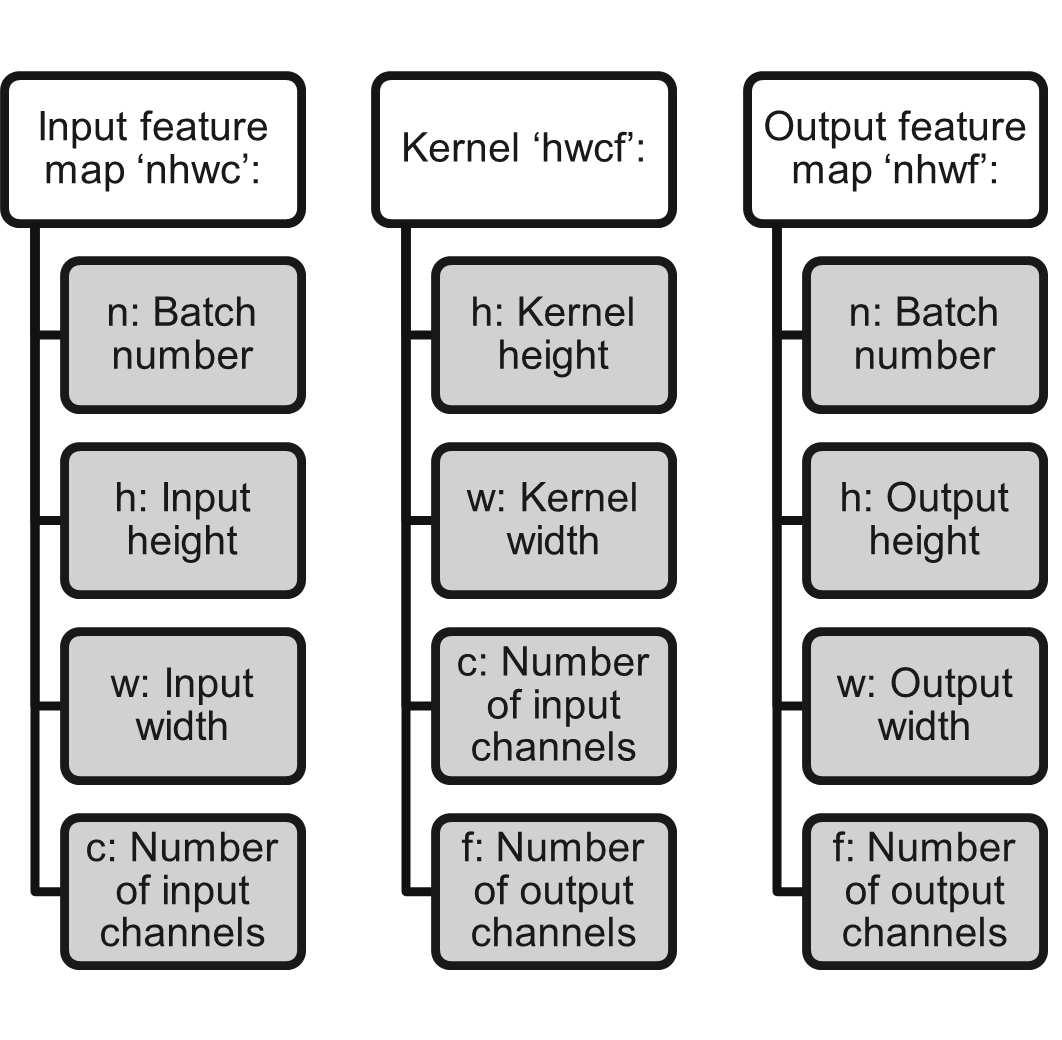
\includegraphics[width=0.5\linewidth]{figure//chapter3_implementation/Figure 2 - conv2d features.png}
    \caption{2D CNN Layer features}
    \label{fig:cnnFeatures}
\end{figure}

\subsubsection{2D Depth-wise Convolution (D-CNN) Layer:}

2D D-CNN layer in MLIR is represented by \textit{'linalg.depthwise\_conv\_2d\_nhwc\_hwc'} as shown in Listing \ref{lst:conv2dLinalg}. The Linalg layer has details such as dilations, strides, input feature map size, kernel size, and output feature map size. Features of the layer are shown in Fig. \ref{fig:dcnnFeatures}

The Listing \ref{lst:dconv2dAffine} shows 6 nested for loops are required for D-CNN layer. The first loop is for batch number. Loop 2 \& 3 are output height and width respectively.  Loop 4 represents number of channels. Loop 5 \& 6 represents kernel height \& width respectively.
\\
\begin{lstlisting}[caption={Example depth-wise conv2d at Linalg dialect}, label={lst:dconv2dLinalg}]
linalg.depthwise_conv_2d_nhwc_hwc 
{dilations = dense<1>: tensor<2xi64>, strides = dense<1>: tensor<2xi64>} 
ins(%arg0, %arg1 : memref<1x32x32x16xf32>, memref<3x3x16xf32>) 
outs(%arg2 : memref<1x30x30x16xf32>)
\end{lstlisting}
\clearpage
\begin{lstlisting}[caption={Example depth-wise conv2d at Affine dialect}, label={lst:dconv2dAffine}]
affine.for %arg3 = 0 to 1 { // Loop 1
  affine.for %arg4 = 0 to 56 {  // Loop 2
    affine.for %arg5 = 0 to 56 {    // Loop 3
      affine.for %arg6 = 0 to 16 {  // Loop 4
        affine.for %arg7 = 0 to 3 { // Loop 5
          affine.for %arg8 = 0 to 3 {   // Loop 6
            ...
\end{lstlisting}

\begin{figure}[H]
    \centering
    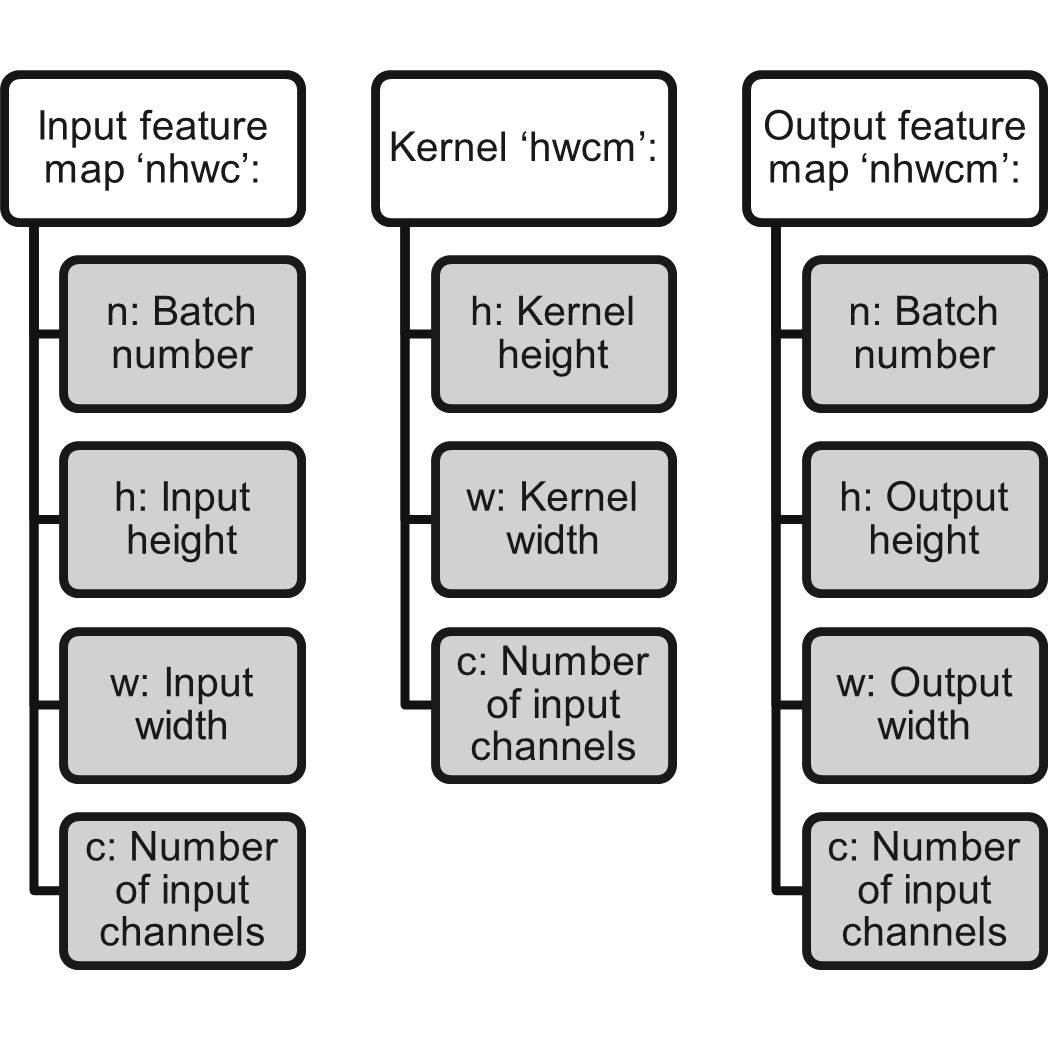
\includegraphics[width=0.5\linewidth]{figure//chapter3_implementation/Figure 3 - dconv2d features.png}
    \caption{D-CNN layer features}
    \label{fig:dcnnFeatures}
\end{figure}


\subsubsection{Fully Connected (FC) Layer:}

FC layer in MLIR is represented by \textit{'linalg.batch\_matmul'} as shown in Listing \ref{lst:fcLinalg}. The Linalg layer has details such as inputs dimensions, weights dimensions, and output dimensions. Features of the layer are shown in Fig. \ref{fig:fcFeatures}

The Listing \ref{lst:fcAffine} shows 4 nested for loops are required for FC layer. The first loop is for batch number. Loop 2 \& 3 are output height and width respectively.  Loop 4 represents kernel height or input width.

\begin{figure}[H]
    \centering
    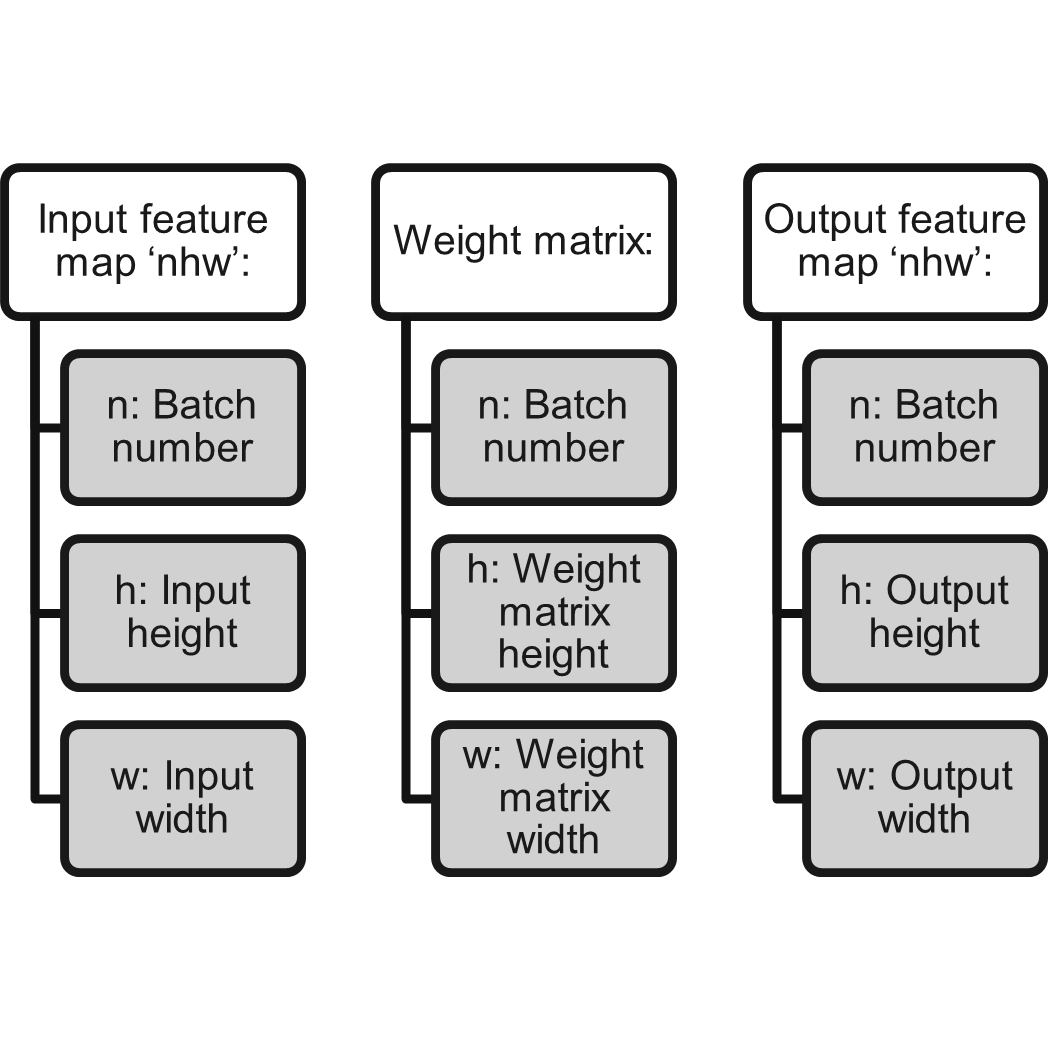
\includegraphics[width=0.5\linewidth]{figure//chapter3_implementation/Figure 4 - fc features.png}
    \caption{FC layer features}
    \label{fig:fcFeatures}
\end{figure}


\begin{lstlisting}[caption={Example depth-wise conv2d at Linalg dialect}, label={lst:fcLinalg}]
linalg.batch_matmul 
ins(%arg0, %arg1 : memref<1x1x9216xf32>, memref<1x9216x4096xf32>) 
outs(%arg2 : memref<1x1x4096xf32>)
\end{lstlisting}

\begin{lstlisting}[caption={Example depth-wise conv2d at Affine dialect}, label={lst:fcAffine}]
affine.for %arg3 = 0 to 1 { // Loop 1
  affine.for %arg4 = 0 to 1 { // Loop 2
    affine.for %arg5 = 0 to 4096 { // Loop 3
      affine.for %arg6 = 0 to 9216 { // Loop 4
        ...
\end{lstlisting}

\clearpage
\subsection{List of Popular Models Explored}

The list of neural network architectures explored is divided into two parts. In the first part, architectures with fewer layers were thoroughly explored, allowing for exhaustive investigation of all possible loop optimization combinations. From this exploration, heuristics were derived based on observed patterns and data analysis. The second part includes larger architectures, where these heuristics were directly applied. For these larger models, the focus was on testing the heuristics to ensure efficient synthesis, achieving near-optimal solutions without the need for exhaustive exploration.
\\
\begin{table}[H]
\caption{Architectures from which heuristic is derived}
\label{tab:architectures1}
\centering
\resizebox{\textwidth}{!}{
\begin{tabular}{|c|c|c|c|c|c|}
\hline
\textbf{No.} & \textbf{Model}        & \textbf{No. of Conv. Layers} & \textbf{No. of D-Conv. Layers} & \textbf{No. of FC Layers} & \textbf{Total No. of layers explored} \\ \hline
1  & \textbf{LeNet} & 3 & NA & 2 & 5 \\ \hline
2  & \textbf{AlexNet} & 5 & NA & 3 & 8 \\ \hline
3  & \textbf{VGG-16} & 13 & - & 3 & 16 \\ \hline
4  & \textbf{MobileNetv3-small} & - & 11 & NA & 11 \\ \hline
 - &  \textbf{Total} & \textbf{21} & \textbf{11} & \textbf{8} & \textbf{40} \\ \hline
\end{tabular}
}
\end{table}

Table \ref{tab:architectures1} presents four architectures: LeNet, AlexNet, VGG-16, and MobileNetV3-Small. A complete exploration of all loop optimization combinations was conducted for LeNet, AlexNet, and MobileNetV3-Small. Based on the observations and patterns identified in LeNet and AlexNet, the search space was narrowed for VGG-16, a comparatively larger architecture, allowing for more targeted optimization. Additionally, VGG-16 played a crucial role in covering all input feature map dimensions for the convolution layer. Following this exploration, heuristics were derived to guide future optimizations, contributing to the comprehensive understanding of convolutional, depthwise convolutional, and fully connected layers across different model complexities.
\\
\begin{table}[H]
\caption{Architectures on which heuristics are tested}
\label{tab:architectures2}
\centering
\resizebox{\textwidth}{!}{
\begin{tabular}{|c|c|c|c|c|c|}
\hline
\textbf{No.} & \textbf{Model}        & \textbf{No. of Conv. Layers} & \textbf{No. of D-Conv. Layers} & \textbf{No. of FC Layers} & \textbf{Total No. of layers explored} \\ \hline
1  & \textbf{VGG-19} & 16 & NA & 3 & 19 \\ \hline
2  & \textbf{Mobilenetv3-large} & - & 15 & NA & 15 \\ \hline
 - &  \textbf{Total} & \textbf{16} & \textbf{15} & \textbf{3} & \textbf{34} \\ \hline
\end{tabular}
}
\end{table}

Table \ref{tab:architectures2} presents two larger architectures—VGG-19 and MobileNetV3-Large—on which direct heuristics were applied without conducting an exhaustive search. Due to the complexity and large number of layers in these models, previously derived heuristics were used to optimize performance, power, and area efficiently. These heuristics were tested on both architectures to determine if they could yield near-optimal results when compared to the actual performance, without needing a full design space exploration. The results were compared to the ground truth to validate the accuracy and effectiveness of the heuristics, ensuring their applicability to larger, more complex architectures.

\subsection{Exploration details}

This section delves into details of configurations generated for loop optimizations.

\subsubsection{Loop permutation:}

\begin{itemize}
    \item CNN layer: It has 72 different permutations to explore. Out of which, 36 are output-first permutations and 36 are kernel-first permutations. Output-first permutation here means that the output's dimensions are placed as the outermost loops, as shown in Listing \ref{lst:conv2dAffineOutputFirst}. Here, loops 2-4 are output's nested for loops. Kernel-first permutation has kernel's dimensions are placed as the outermost loops, as shown in Listing \ref{lst:conv2dAffineKernelFirst}. Here, loops 2-4 are kernel's nested for loops.
    \item D-CNN layer: Similar to CNN layer, this has 24 different permutations to explore. Out of which 12 are output first permutations, as shown in \ref{lst:dconv2dAffineOutputFirst}. Here, loops 2-4 are output's nested for loops. The other 12 are kernel first permutations, as shown in \ref{lst:dconv2dAffineKernelFirst}. Here, loops 2-4 are kernel's nested for loops.
    \item FC layer: This layer has 6 different permutations to explore.
\end{itemize}

\begin{lstlisting}[caption={Example conv2d with output-first permutation}, label={lst:conv2dAffineOutputFirst}]
affine.for %arg3 = 0 to 1 { // Loop 1
  affine.for %arg4 = 0 to 55 { // Loop 2
    affine.for %arg5 = 0 to 55 { // Loop 3
      affine.for %arg6 = 0 to 96 { // Loop 4
        affine.for %arg7 = 0 to 11 { // Loop 5
          affine.for %arg8 = 0 to 11 { // Loop 6
            affine.for %arg9 = 0 to 3 { // Loop 7
                .....
\end{lstlisting}
\begin{lstlisting}[caption={Example conv2d with kernel-first permutation}, label={lst:conv2dAffineKernelFirst}]
affine.for %arg3 = 0 to 1 { // Loop 1
  affine.for %arg4 = 0 to 11 { // Loop 2
    affine.for %arg5 = 0 to 11 { // Loop 3
      affine.for %arg6 = 0 to 3 { // Loop 4
        affine.for %arg7 = 0 to 55 { // Loop 5
          affine.for %arg8 = 0 to 55 { // Loop 6
            affine.for %arg9 = 0 to 96 { // Loop 7
                .....
\end{lstlisting}

\begin{lstlisting}[caption={Example depth-wise conv2d at Affine dialect}, label={lst:dconv2dAffineOutputFirst}]
affine.for %arg3 = 0 to 1 { // Loop 1
  affine.for %arg4 = 0 to 56 {  // Loop 2
    affine.for %arg5 = 0 to 56 {    // Loop 3
      affine.for %arg6 = 0 to 16 {  // Loop 4
        affine.for %arg7 = 0 to 3 { // Loop 5
          affine.for %arg8 = 0 to 3 {   // Loop 6
            ...
\end{lstlisting}
\clearpage
\begin{lstlisting}[caption={Example depth-wise conv2d at Affine dialect}, label={lst:dconv2dAffineKernelFirst}]
affine.for %arg3 = 0 to 1 { // Loop 1
  affine.for %arg4 = 0 to 3 {  // Loop 2
    affine.for %arg5 = 0 to 3 {    // Loop 3
      affine.for %arg6 = 0 to 16 {  // Loop 4
        affine.for %arg7 = 0 to 56 { // Loop 5
          affine.for %arg8 = 0 to 56 {   // Loop 6
            ...
\end{lstlisting}

\subsubsection{Loop tiling:}
\begin{itemize}
    \item CNN or D-CNN layer: For 2D Convolution and 2D Depth-wise Convolution layer's output height/width, kernel height/width and input\_channels are tiled in powers of 2 from 4 to the maximum dimension. If the dimension has a value under 4, then only 1 combination (maximum possible dimension) is explored. 
    \item FC layer: For FC layer, output height, output width, and kernel width are tiled in powers of 2 from 4 to the maximum dimension.
\end{itemize}


\subsubsection{Loop unrolling:}
\begin{itemize}
    \item CNN or D-CNN layer: For 2D Convolution and 2D Depth-wise Convolution layers with no. of unrolls 1, 2, and 3 with factors 4, 8, 16, until full-unroll are performed.
    \item FC layer: For FC layer with no. of unrolls 1 and 2 with factors 4, 8, 16, and full-unroll are performed.

\end{itemize}

\clearpage
\subsection{HLS parameters}

\begin{table}[h!]
\caption{HLS parameters}
\centering
\label{tab:hlsParameters}
\begin{tabular}{|c|c|c|}
\hline
\textbf{Configuration} & \textbf{Values} \\ \hline
\textbf{Maximum clock cycles} & $2^{32} - 1$ \\ \hline
\textbf{Frequency} & 100 MHz \\ \hline
\textbf{Memory allocation policy} & NO\_BRAM \\ \hline
\textbf{PDK} & NanGate45 \\ \hline
\end{tabular}
\end{table}

The Table \ref{tab:hlsParameters} outlines key configuration parameters used in High-Level Synthesis (for Bambu). The final ASIC generated depends a lot on frequency, Process Design Kit (PDK), and memory allocation policies. Here's the list of reasons to select these values:

\begin{itemize}
    
    \item Maximum clock cycles: It is set to $2^{32} - 1$, which represents the maximum allowable number of clock cycles in the test-bench generated by Bambu. This large value accommodates extended operations, ensuring that the system can handle very large designs without prematurely terminating.

    \item Frequency: At a frequency of 100 MHz, the system is tuned to avoid any timing violations. This frequency is chosen to balance performance and stability, so that no critical path timing violations occur during execution. Timing violations can disrupt synchronization or various hardware components, leading to failures. Therefore, this frequency was selected to ensure stable operation across all modules.

    \item Memory allocation policy: The memory allocation policy is set to NO\_BRAM, indicating that memory modules should not be synthesized. Memory, like Block-RAM (BRAM) is typically placed as macros within ASICs. These macros are pre-defined, optimized circuits created using memory compilers. These macros then need to efficiently integrated into final design.

    \item Process Design Kit (PDK): PDK used to create ASIC in this DSE in NanGate45. It is a widely-used open-source PDK for 45nm technology nodes. The PDK provides necessary design rules, standard cell libraries, and technology files required for ASIC synthesis and physical design. NanGate45 is often chosen for research and academic purposes due to its accessibility and comprehensive support for modern design flows.
    
\end{itemize}

\clearpage
\section{Refinements in DSE Methodology}

This section presents refinements made in SODA framework and modifications to the neural network layer's dimensions aimed at alleviating bottlenecks. Additionally, key challenges faced during loop optimizations are highlighted and potential solutions are discussed.

\subsection{SODA}

\begin{figure}[H]
    \centering
    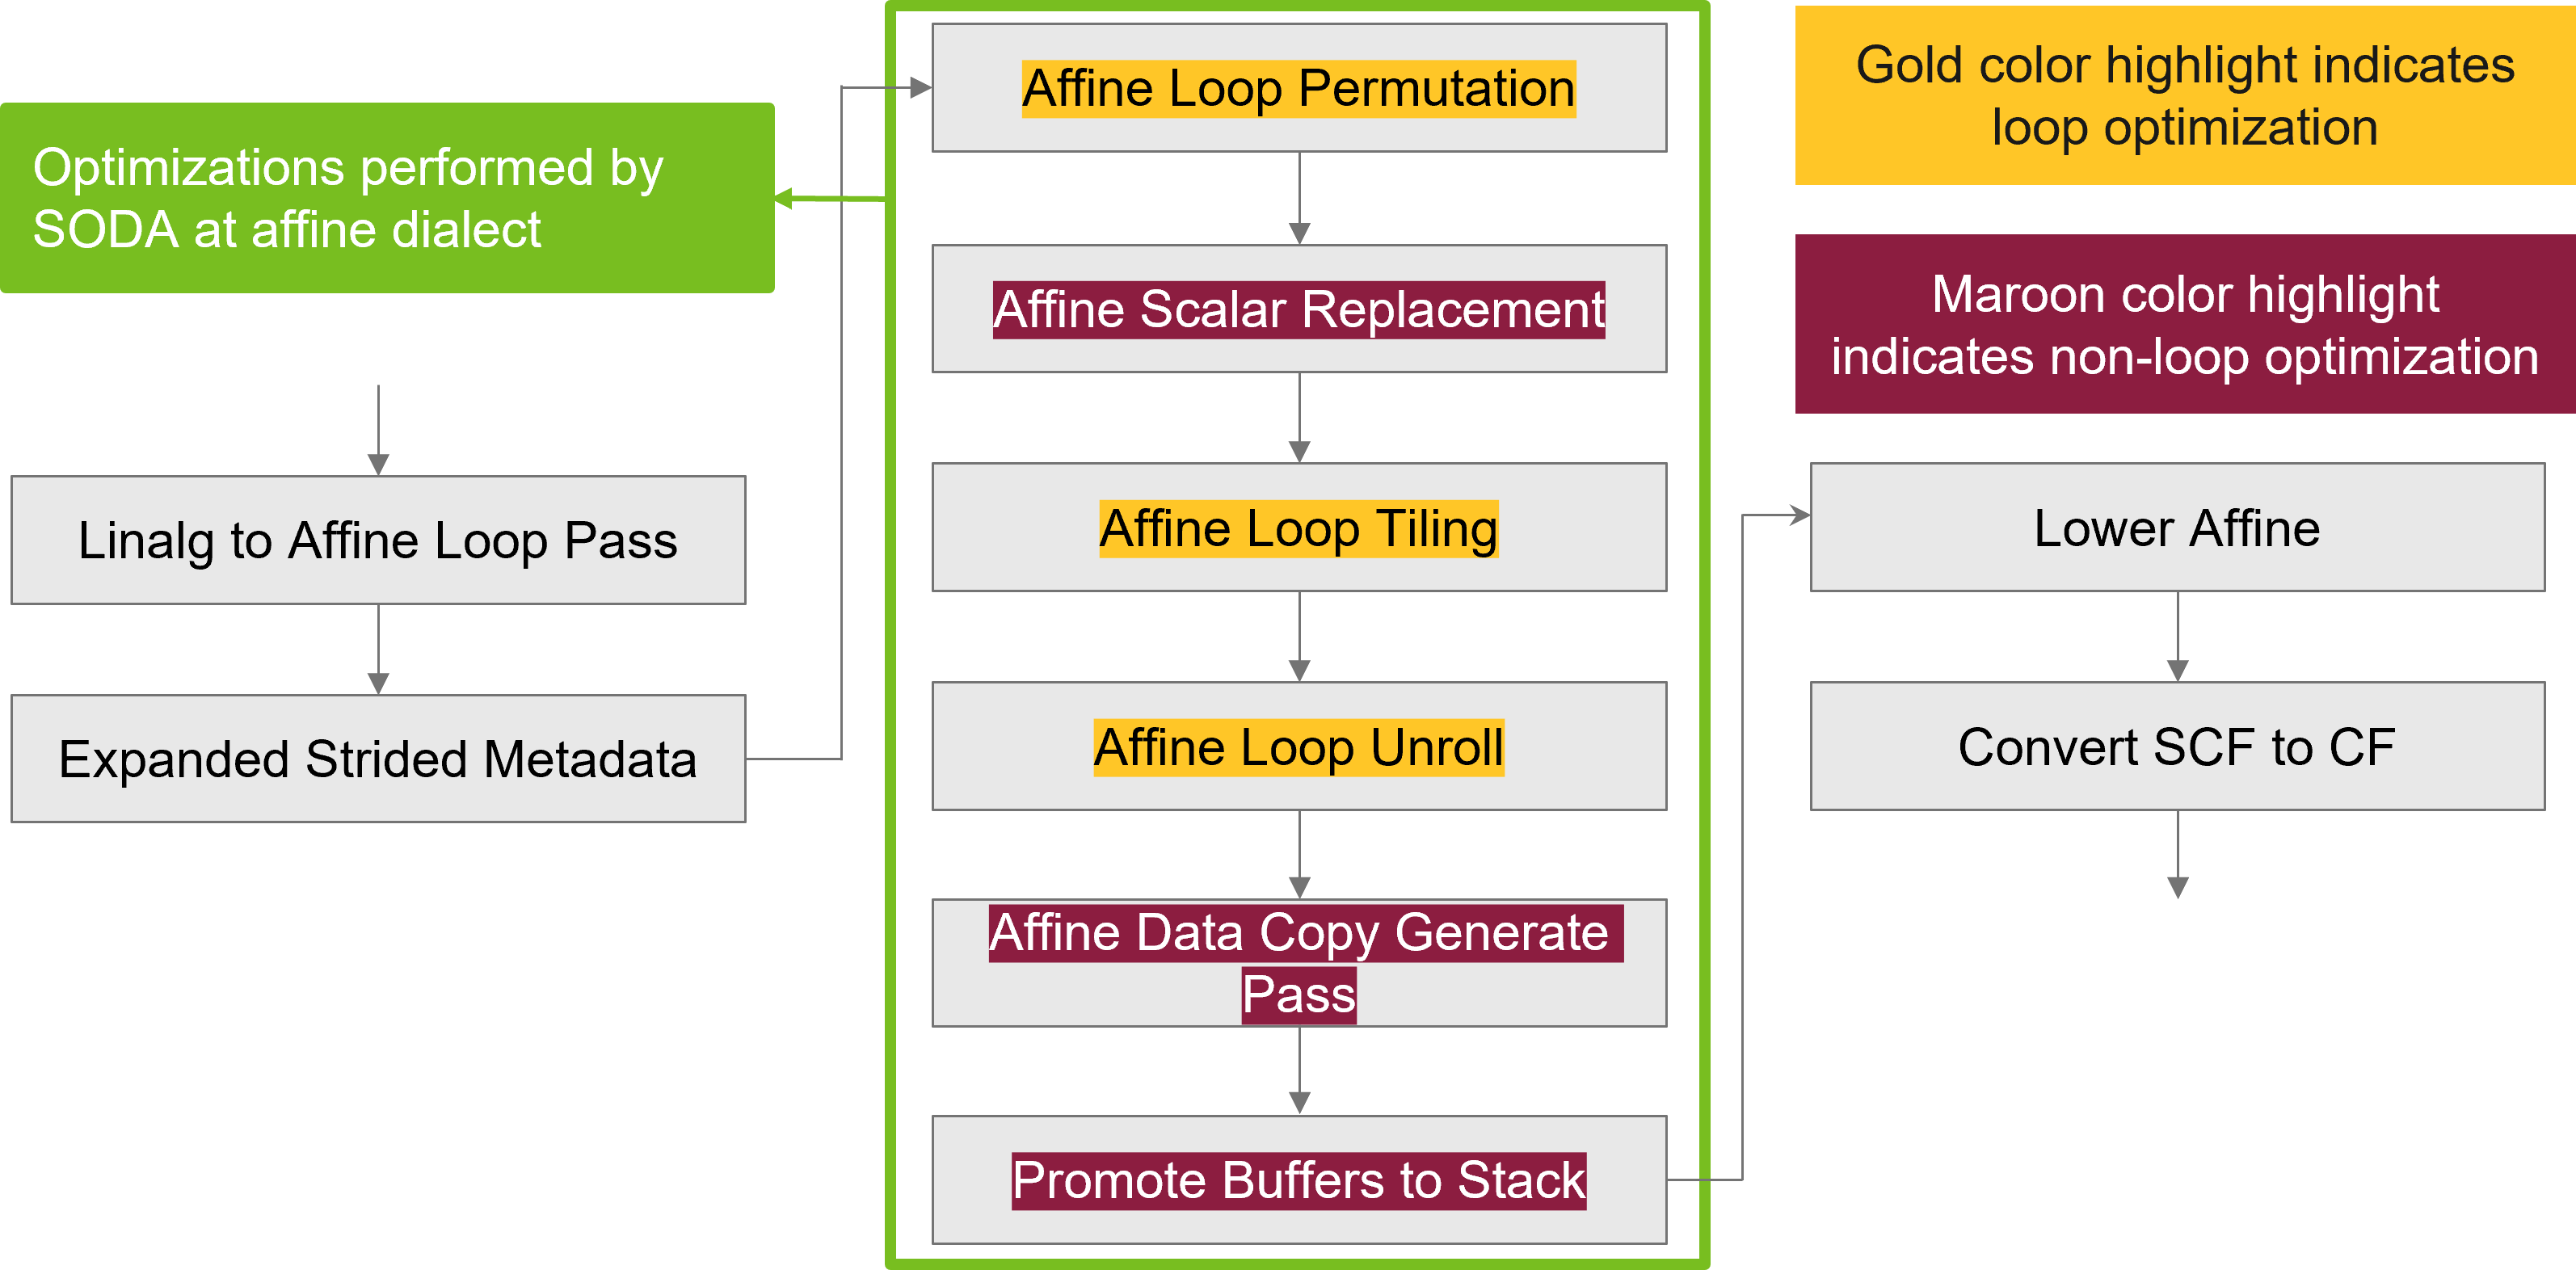
\includegraphics[width=1\linewidth]{figure//chapter3_implementation/Figure 5 - refined soda.png}
    \caption{Refined SODA pipeline for Bambu}
    \label{fig:refinedSODA}
\end{figure}

The thought procedure behind applying loop optimizations involves a structured and sequential approach to ensure maximum performance gains while minimizing complexity. Here's a list of key steps to follow:

\begin{itemize}
    
    \item Perform Affine Scalar Replacement before loop unrolling: Scalar replacement is an essential optimization that replaces memory loads and stores with register accesses for scalar variables. By applying affine scalar replacement before loop unrolling, you ensure that scalar values are moved to faster register memory in a smaller loop body. This avoids the added complexity of managing scalar values after unrolling, where handling expanded loops can lead to redundant memory accesses. Performing scalar replacement early ensures the loop is already optimized for memory access when the loop body is unrolled, allowing for better overall efficiency.

    \item Perform Affine data copy generation after loop unrolling: The affine data copy generation pass is responsible for managing the movement of data between memory buffers, optimizing how data is stored and retrieved within loops. By running this pass after loop unrolling, you prevent unnecessary expansion of buffer storage loops, which would occur if done beforehand. Waiting unroll after unrolling ensures more streamlined memory operations and avoids unnecessary buffer management in expanded loop structure.

    \item Perform loop optimizations in the order of permutation, tiling, and unrolling: A strategic order of applying loop optimizations is to start with permutation, followed by tiling, and finally unrolling. This simplifies the process of combining multiple optimizations. Loop permutation, which rearranges loop nests to improve data locality. Once the loops are structured optimally, tiling divides them into smaller, memory-friendly blocks, ensuring they fit within a memory block. This improves memory utilization and, as a result, enhances performance. Unrolling is then applied to further enhance parallelism and reduce loop overhead. Following this sequence ensures that each optimization builds upon the previous one, making the combined effects more impactful and easier to manage.
\end{itemize}

\subsection{Optimizations}
\subsubsection{Loop permutation:}
Permutation mapping in MLIR-OPT has been identified as a source of issues, as it does not work correctly. Specific permutation mapping mistakes were discovered in several operations, including \textit{'linalg.batch\_matmul'}, \textit{'linalg.conv2d\_nhwc\_hwcf'}, and \\ \textit{'linalg.depthwise\_conv\_2d\_nhwc\_hwc'}. To address these issues and ensure correct mapping, CSV files were created for all three linalg operations, providing a solution for proper permutation mapping.


\begin{table}[h]
\caption{Statistics of Permutation Mapping for Different Layer Types}
\label{tab:permStats}
\centering
\resizebox{\textwidth}{!}{%
\begin{tabular}{|l|c|c|c|}
\hline
\textbf{Layer Type} & \textbf{No. of permutations that map correctly} & \textbf{Total No. of permutations} & \textbf{\% of correctly mapped permutations} \\ \hline
\texttt{linalg.conv2d\_nhwc\_hwcf} & 22 & 72 & 30.56\% \\ \hline
\texttt{linalg.depthwise\_conv\_2d\_nhwc\_hwc} & 10 & 24 & 41.67\% \\ \hline
\texttt{linalg.batch\_matmul} & 4 & 6 & 66.67\% \\ \hline
\textbf{Total:} & 36 & 102 & 35.30\% \\ \hline
\end{tabular}
}
\end{table}

As the Table \ref{tab:permStats} demonstrates, the percentage of correctly mapped permutations varies across layer types. In the case of \textit{'linalg.conv2d\_nhwc\_hwcf'}, only 30.56\% of the attempted permutations were correctly mapped, indicating the need for more refinement in mapping for this layer. For \textit{'linalg.depthwise\_conv\_2d\_nhwc\_hwc'}, the percentage of correct mappings is higher at 41.67\%, but there is still room for improvement. \textit{'linalg.batch\_matmul'} shows the highest percentage, with 66.67\% of permutations mapping correctly, indicating that the permutation mapping process works more effectively for this layer.

The overall percentage of correct mappings across all layers is 35.30\%, underscoring the importance of refining permutation strategies to achieve higher accuracy in mapping permutations across different neural network operations.

\begin{table}[H]
\caption{Permutation attempts and their outcomes for \textit{'linalg.batch\_matmul'}}
\label{tab:matmulPermutation}
\centering
\begin{tabular}{|c|c|c|}
\hline
\textbf{Permutation No.} & \textbf{Permutation tried} & \textbf{Does it work?} \\ \hline
1 & 0,1,2,3 & Yes \\ \hline
2 & 0,1,3,2 & Yes \\ \hline
3 & 0,2,1,3 & Yes \\ \hline
4 & 0,2,3,1 & No (This maps to 0,3,1,2) \\ \hline
5 & 0,3,1,2 & No (This maps to 0,2,3,1) \\ \hline
6 & 0,3,2,1 & Yes \\ \hline
\end{tabular}%
\end{table}


As an example, the Table \ref{tab:matmulPermutation} illustrates different permutations that were tried. For permutations like 0,1,2,3 (Permutation No. 1) and 0,1,3,2 (Permutation No. 2), the mapping worked successfully. However, for other cases such as 0,2,3,1 (Permutation No. 4), it did not work and incorrectly mapped to 0,3,1,2. Similar issues were found with permutation 0,3,1,2 (Permutation No. 5), which mapped to 0,2,3,1. These examples demonstrate the importance of precise permutation mapping, and the CSV files help resolve these issues by ensuring proper mapping across various operations.

\subsubsection{Loop unrolling:}

For loop unrolling, two main issues arise. The first issue involves Affine Scalar Replacement, which can cause significant delays if performed before the loop unrolling process. If scalar replacement is applied too early, it takes considerable time to replace all scalars in the unrolled affine loop. To address this, it is recommended to perform affine loop unrolling after the scalar replacement process, ensuring efficiency in handling scalars within the unrolled loops.

The second issue revolves around the Buffer Trick, where temporary buffers are used to store intermediate values. While this technique allows data in the buffers to be accessed quickly, it creates an excess of buffers when combined with loop unrolling. This can complicate the synthesis process, particularly when using tools like Bambu to generate Verilog code. To avoid these complications, it is recommended to remove the buffer trick for unrolling, simplifying the number of buffers and streamlining the synthesis process.

\subsubsection{Loop tiling:}

One of the key issues encountered during loop tiling is related to the "Promote Buffers to Stack" pass. This pass causes the affine loop tiling pass to fail, throwing an error. To resolve this, the recommendation is to remove the "Promote Buffers to Stack" pass entirely. By doing so, the affine loop tiling pass can execute without errors, ensuring that the tiling optimizations can be successfully applied to the loops in question.

\subsection{Neural Network Layers}

\subsubsection{Clipping dimensions:}

Clipping the dimensions of neural network layers addresses two key bottlenecks in hardware design and simulation.
\begin{enumerate}
    \item The first bottleneck arises from the challenge of designing ASICs for large neural network. As the size of the network increases, the power consumption and area required for the ASIC also scale significantly, making the design costly and impractical for manufacturing. By clipping the dimensions of the neural network layers, the design's power and area requirements are reduced, ultimately lowering the cost and complexity of producing the ASIC.
    \item The second bottleneck is caused by simulation constraints imposed by Bambu. Bambu's test-bench imposes a limit on the number of clock cycles that can be simulated for a given design. Without dimensions clipping, larger neural networks may exceed this clock cycle limit, making them not synthesizable to ASIC. Clipping dimensions ensures that design remains within the maximum allowable clock cycles, enabling successful simulation while staying within test-bench's constraints.
\end{enumerate}

\begin{table}[H]
\caption{Input feature map height/width and Max Input channels}
\label{tab:clipInput}
\centering
\begin{tabular}{|c|c|}
\hline
\textbf{Input feature map height/width} & \textbf{Maximum no. of Input channels} \\ \hline
$\leq 16$ & 128 \\ \hline
$> 16$ and $\leq 32$ & 32 \\ \hline
$> 32$ and $\leq 64$ & 8 \\ \hline
$> 64$ & 1 \\ \hline
\end{tabular}
\end{table}

For 2D Convolution and Depth-wise 2D convolution layers, output channels are clipped to 1, and input channels are clipped based on the input feature map height/width, as shown in Table \ref{tab:clipInput}. This ensures efficient convolution operations while maintaining test accuracy.
\\
\begin{table}[H]
\caption{CNN layers clipping for unrolling based on input feature map and kernel size}
\label{tab:clipInputUnroll}
\centering
\resizebox{\textwidth}{!}{%
\begin{tabular}{|c|c|c|}
\hline
\textbf{Input feature map height/width} & \textbf{Kernel height/width} & \textbf{Maximum no. of input channels} \\ \hline
\multirow{4}{*}{$\leq 64$} & $\leq 3$ & 32 \\ \cline{2-3} 
                           & $> 3$ and $\leq 5$ & 8 \\ \cline{2-3} 
                           & $> 5$ and $\leq 7$ & 4 \\ \cline{2-3} 
                           & $> 7$ & 1 \\ \hline
$> 64$                     & $1 - 11$ & 1 \\ \hline
\end{tabular}
}
\end{table}

Table \ref{tab:clipInputUnroll} further shows how CNN layer clipping for unrolling depends on kernel size and input feature map dimensions, which determine the maximum input channels. For example, with input maps $\leq 64$ and kernel size $\leq 3$, up to 32 input channels are supported, with larger kernel sizes progressively reducing this limit.

Finally, to estimate the total number of clock cycles required to process an entire layer, the number of simulation cycles for processing a single tile is multiplied by the total number of tiles in the layer. This estimation approach ensures that computational resources are optimized for the entire process.


\begin{figure}[H]
    \centering
    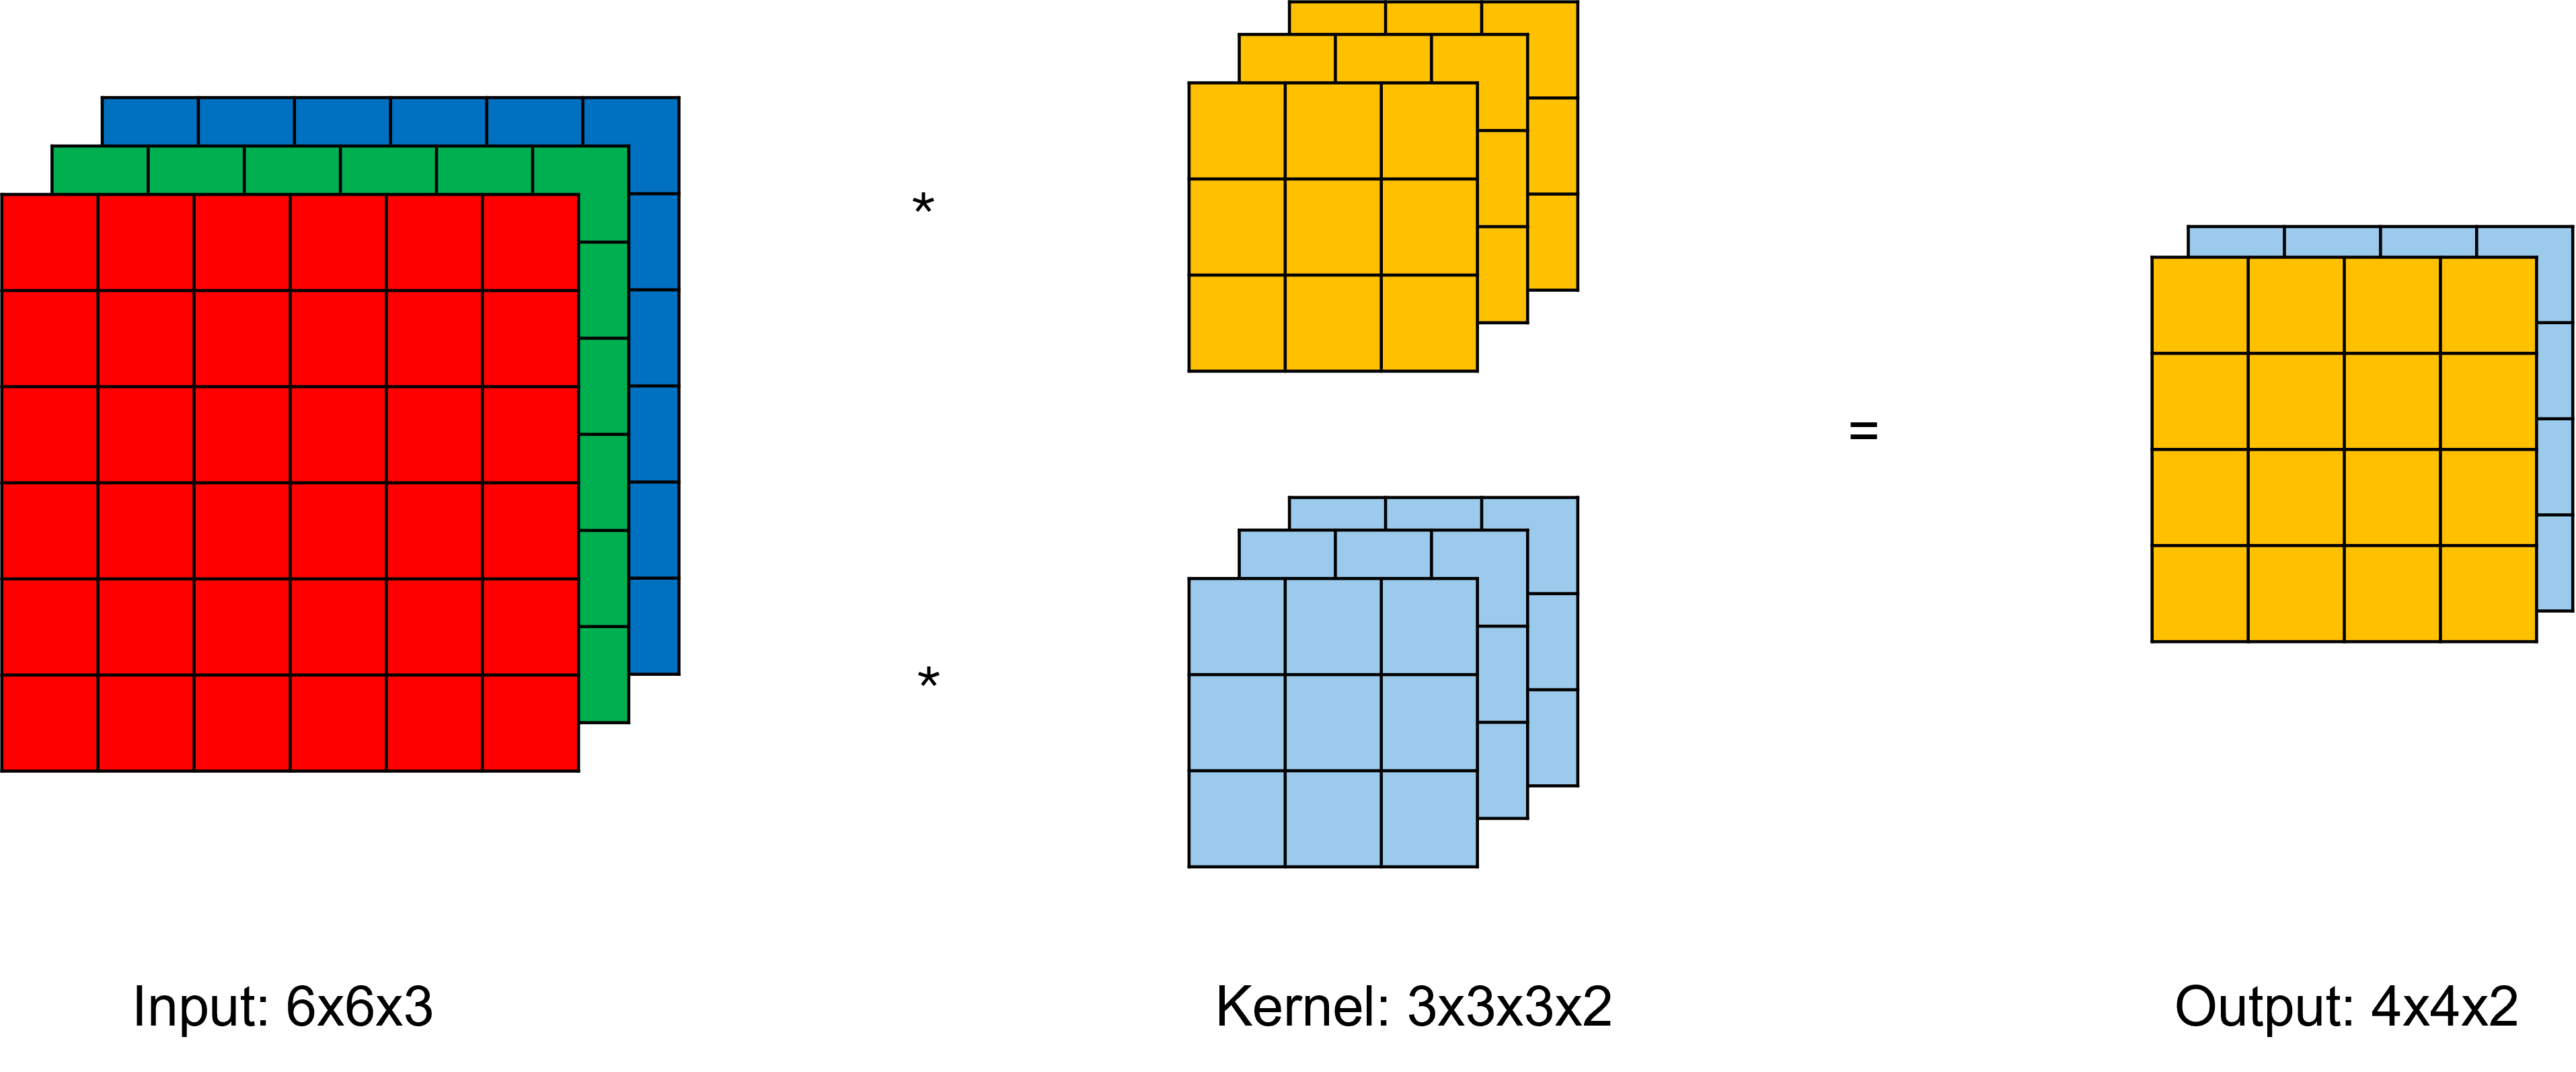
\includegraphics[width=0.7\linewidth]{figure//chapter3_implementation/Figure 6 - output channels 2.png}
    \caption{CNN Layer with 2 output channels}
    \label{fig:2OpCh}
\end{figure}

\begin{figure}[H]
    \centering
    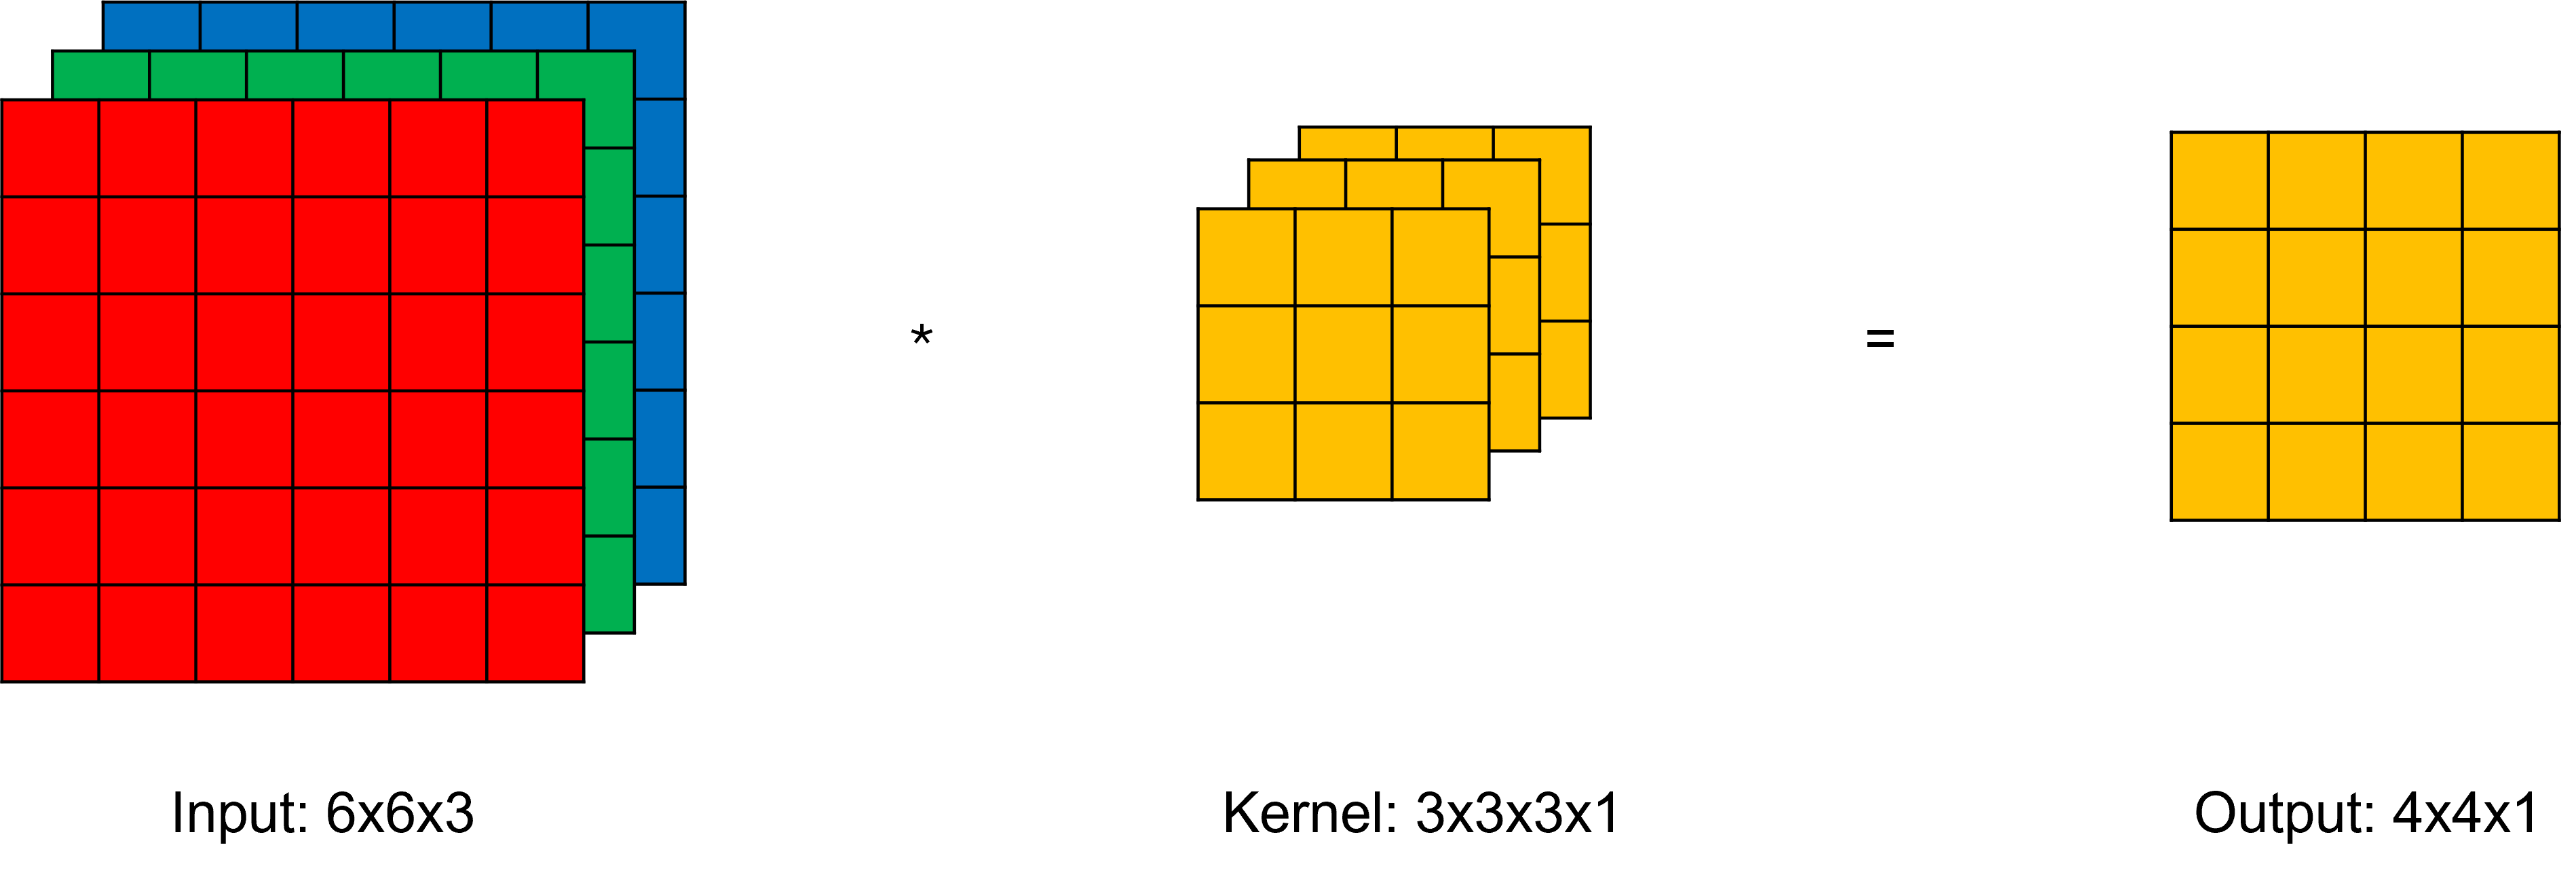
\includegraphics[width=0.7\linewidth]{figure//chapter3_implementation/Figure 7 - output channels 1.png}
    \caption{CNN Layer with 1 output channel}
    \label{fig:1OpCh}
\end{figure}

For example, consider a neural network layer where the actual number of output channels are 2, as shown in Figure \ref{fig:2OpCh}. Due to limitations such as Bambu's test-bench constraints on the number of clock cycles, or in the case where producing the design would result in an excessively large ASIC, simulating the entire layer directly is not feasible. To address this, clipping dimensions are applied, reducing the number of output channels, as illustrated in Figure \ref{fig:1OpCh}. This allows us to simulate the network within Bambu’s constraints or design a smaller, more manageable ASIC. To estimate the number of clock cycles required for simulating 2 output channels, we simply multiply the number of clock cycles needed for 1 output channel by 2, providing an approximate value.

\subsubsection{Depth-wise Convolution (D-CNN) mapping:}

During the mapping of the Depth-wise Convolutional Neural Network (D-CNN) to \\ \textit{'linalg.depthwise\_conv\_2d\_nhwc\_hwcm'}, as shown in Listing \ref{lst:dconv2d_hwc} at Affine level, it became evident that certain loop optimizations, such as loop unrolling, were not performing optimally. To overcome this, the layer was instead mapped to \textit{'linalg.depthwise\_conv\_2d\_nhwc\_hwc'}, as illustrated in Listing \ref{lst:dconv2d_hwc}. This alternative mapping not only enhanced optimization performance but also promoted uniformity. Given that most popular neural network architectures commonly use a depth multiplier of 1, mapping directly to \textit{'linalg.depthwise\_conv\_2d\_nhwc\_hwc'} ensures consistency across various models.

\begin{lstlisting}[caption={Example depth-wise conv2d at Affine dialect}, label={lst:dconv2d_hwcm}]
affine.for %arg3 = 0 to 1 { // Loop 1
  affine.for %arg4 = 0 to 56 {  // Loop 2
    affine.for %arg5 = 0 to 56 {    // Loop 3
      affine.for %arg6 = 0 to 16 {  // Loop 4
        affine.for %arg7 = 0 to 1 { // Loop 5
            affine.for %arg7 = 0 to 3 { // Loop 6
                affine.for %arg8 = 0 to 3 {   // Loop 7
                    ...
\end{lstlisting}

\begin{lstlisting}[caption={Example depth-wise conv2d at Affine dialect}, label={lst:dconv2d_hwc}]
affine.for %arg3 = 0 to 1 { // Loop 1
  affine.for %arg4 = 0 to 56 {  // Loop 2
    affine.for %arg5 = 0 to 56 {    // Loop 3
      affine.for %arg6 = 0 to 16 {  // Loop 4
        affine.for %arg7 = 0 to 3 { // Loop 5
          affine.for %arg8 = 0 to 3 {   // Loop 6
            ...
\end{lstlisting}
